\section{Dormand-Prince (DOPRI54)}
\subsection{DOPRI54 with adaptive step size}
A special case of Runge-Kutta methods is the Dormand-Price. So relating to the general Runge-Kutta formulas in equation \ref{eq:RKgeneral1} and \ref{eq:RKgeneral2}, the Dormand-Prince method is obtained by choosing coefficients summarised by the following Butchers Tableau \cite{JrgensenRunge-KuttaEquations}:

\begin{table}[H]
\centering
%\caption{}
%\label{tab:q6_ButcherDOPRI54}
\begin{tabular}{c|ccccccc}
0 & 0 & 0 & 0 & 0 & 0 & 0 & 0 \\
$\frac{1}{3}$ & $\frac{1}{5}$ & 0 & 0 & 0 & 0 & 0 & 0 \\
$\frac{3}{10}$ & $\frac{3}{40}$ & $\frac{9}{40}$ & 0 & 0 & 0 & 0 & 0 \\
$\frac{4}{5}$ & $\frac{44}{45}$ & $\frac{-56}{15}$ & 0 & 0 & 0 & 0 & 0 \\
$\frac{8}{9}$ & $\frac{19372}{6561}$ & $\frac{-25360}{2187}$ & $\frac{64448}{6561}$ & $\frac{-212}{729}$ & 0 & 0 & 0 \\
1 & $\frac{9017}{3168}$ & $\frac{-355}{33}$ & $\frac{46732}{5247}$ & $\frac{49}{176}$ & $\frac{-5103}{18656}$ & 0 & 0 \\
1 & $\frac{35}{384}$ & 0 & $\frac{500}{1113}$ & $\frac{125}{192}$ & $\frac{-2187}{6784}$ & $\frac{11}{84}$ & 0 \\ \hline
 $x$ &  $\frac{35}{384}$ & 0 & $\frac{500}{1113}$ & $\frac{125}{192}$ & $\frac{-2187}{6784}$ & $\frac{11}{84}$ & 0  \\
$\hat{x}$ & $\frac{5179}{57600}$ & 0 & $\frac{7571}{16695}$ & $\frac{393}{640}$ & $\frac{-92079}{339200}$ & $\frac{187}{2100}$ & $\frac{1}{40}$ \\ \hline
$e$ & $\frac{71}{57600}$ & 0 & $\frac{-71}{16695}$ & $\frac{71}{1920}$ & $\frac{-17253}{339200}$ & $\frac{22}{525}$ & $\frac{-1}{40}$
\end{tabular}%
\caption{Butchers Tableau of DOPRI54.}
\end{table}

In other words, it has 7 stages and it is a 5th order method with a 4th order embedded method for error estimation. This means that the error the method commits from the exact solution is estimated by the difference between the 4th order solution from the more accurate 5th order solution: $e_n = x_n - \hat{x}_n = \Delta t_k \sum_{j=1}^{s} d_{j} f\left(T_{j}, X_{j}\right)$. The step size $\Delta t_n$ is then iteratively updated by

\begin{equation}
\Delta t_{n+1, j}=\left(\frac{\epsilon}{r_{n+1, j}}\right)^{\frac{1}{5}} \Delta t_{n, j}
\end{equation}

Over iterations of \textit{j}, until $r_{n+1, j} \leq 1$ where the step size is passed on $\Delta t_{n+1} = \Delta t_{n+1, j_{r\leq1}}$. $r_{n+1}$ is then calculated as
\begin{equation}
    r_{n+1} = \left\|e_{n+1}\right\|_\infty = \max _{p \in\{1, \ldots, P\}} \frac{\left|e_{p}\right|}{\mathrm{abs}_{p}+\left|x_{p}\right| \mathrm{rel}_{p}}
\end{equation}

Where \textit{P} is the dimension of $\boldsymbol{x}$. In this report, $\mathrm{abs}_p = \mathrm{rel}_p \quad \forall_p$ will be used.




Often the power used is $\frac{1}{p+1}$ for when the embedded method is the one of highest order. However in this case the embedded method is of order 4 and therefore $\frac{1}{4+1}$ is used. \\
Since it is a 5th order method the local approximations error $l_n \propto (\Delta t_n)^{6}$.

\subsection{MATLAB implementation adaptive step size}
The following listing implements the DOPRI54 as described in the previous section.

\begin{adjustwidth*}{0cm}{-0.4cm}
\begin{lstlisting}[frame=single, language=Matlab,caption=DOPRI54, label=ERKpars]
function [Tout,Xout,Eout] = ...
        DOPRI54Adaptive(fun,tspan,x0,h,solver, ...
        abstol, reltol, varargin)

% Epsilon tolerance
epstol=0.8;

% DOPRI54 coefficients 
s = 7;
A = zeros(s,s);
A(2,1) = 1/5;
A(3,1) = 3/40;
A(4,1) = 44/45;
A(5,1) = 19372/6561;
A(6,1) = 9017/3168;
A(7,1) = 35/384;
A(3,2) = 9/40;
A(4,2) = -56/15;
A(5,2) = -25360/2187;
A(6,2) = -355/33;
A(4,3) = 32/9;
A(5,3) = 64448/6561;
A(6,3) = 46732/5247;
A(7,3) = 500/1113;
A(5,4) = -212/729;
A(6,4) = 49/176;
A(7,4) = 125/192;
A(6,5) = -5103/18656;
A(7,5) = -2187/6784;
A(7,6) = 11/84;
AT = A'
%bhat = [5179/57600; 0; 7571/16695; 393/640; -92097/339200; 187/2100; 1/40];
b = [35/384; 0; 500/1113; 125/192; -2187/6784; 11/84; 0];
c = [0; 1/5; 3/10; 4/5; 8/9; 1; 1];
d = [71/57600; 0; -71/16695; 71/1920; -17253/339200; 22/525; -1/40];
o = 5; % Order p=5
kpow  = 1/(o);     % Usually: kpow = 1/(order + 1)

h = h; % INIT

% Size parameters
x  = x0;                % Initial state
t  = tspan(1);          % Initial time
tf = tspan(end);        % Final time
nx = length(x0);        % System size (dim(x))

% Allocate memory
T  = zeros(1,s);        % Stage T
X  = zeros(nx,s);       % Stage X
F  = zeros(nx,s);       % Stage F

% More init
Tout = t;        
Xout = x';
Eout = 0;

% Algorithm starts here
while t < tf
    if (t+h > tf) % Don't go to far
        h = tf-t;
    end

    AcceptStep = false;
    while ~AcceptStep
        %%% Runge-Kutta
        % Stage 1
        T(1)   = t;
        X(:,1) = x;
        F(:,1) = fun(T(1),X(:,1),varargin{:});
        
        % Stage 2,3,...,s
        T(2:s) = t + h*c(2:s);
        for i=2:s
            X(:,i) = x + F(:,1:i-1)*h*AT(1:i-1,i);
            F(:,i) = feval(fun,T(i),X(:,i),varargin{:});
        end

        % Estimate of apprixmation error
        e = F*h*d;

        % Controlling step size h relative to error
        r = max(abs(e) ./ max(abstol, abs(x + F*h*b) .*reltol));
        h = (epstol/r)^(kpow) * h;

        AcceptStep = (r<=1.0);
        if AcceptStep
            t = t+h;
            x = x + F*h*b;
        end
    end
    % Save output when AcceptStep == true
    Tout = [Tout; t];
    Xout = [Xout; x'];
    Eout = [Eout; e];
end
\end{lstlisting}
\end{adjustwidth*}



\subsection{Test equation, order \& stability}
Considering again the test equation

$$
\dot{x}(t)=\lambda x(t), \quad x(0)=x_{0} \label{eq:test}
$$
With the analytical solution
$$
x(t) = \exp(\lambda t)
$$

And choosing $\lambda=-1$ and $x_{0}=1$ the approximated solutions as obtained by DOPRI54 is seen in Figure \ref{fig:6_3}. For a high tolerance the solution is quite off and with a decreasing tolerance the solution approaches that of the exact, analytical solution. Note how the DOPRI54 is not only far off the right solution, its embedded error estimation is also far off.

\begin{figure}[htb]
    \centering
    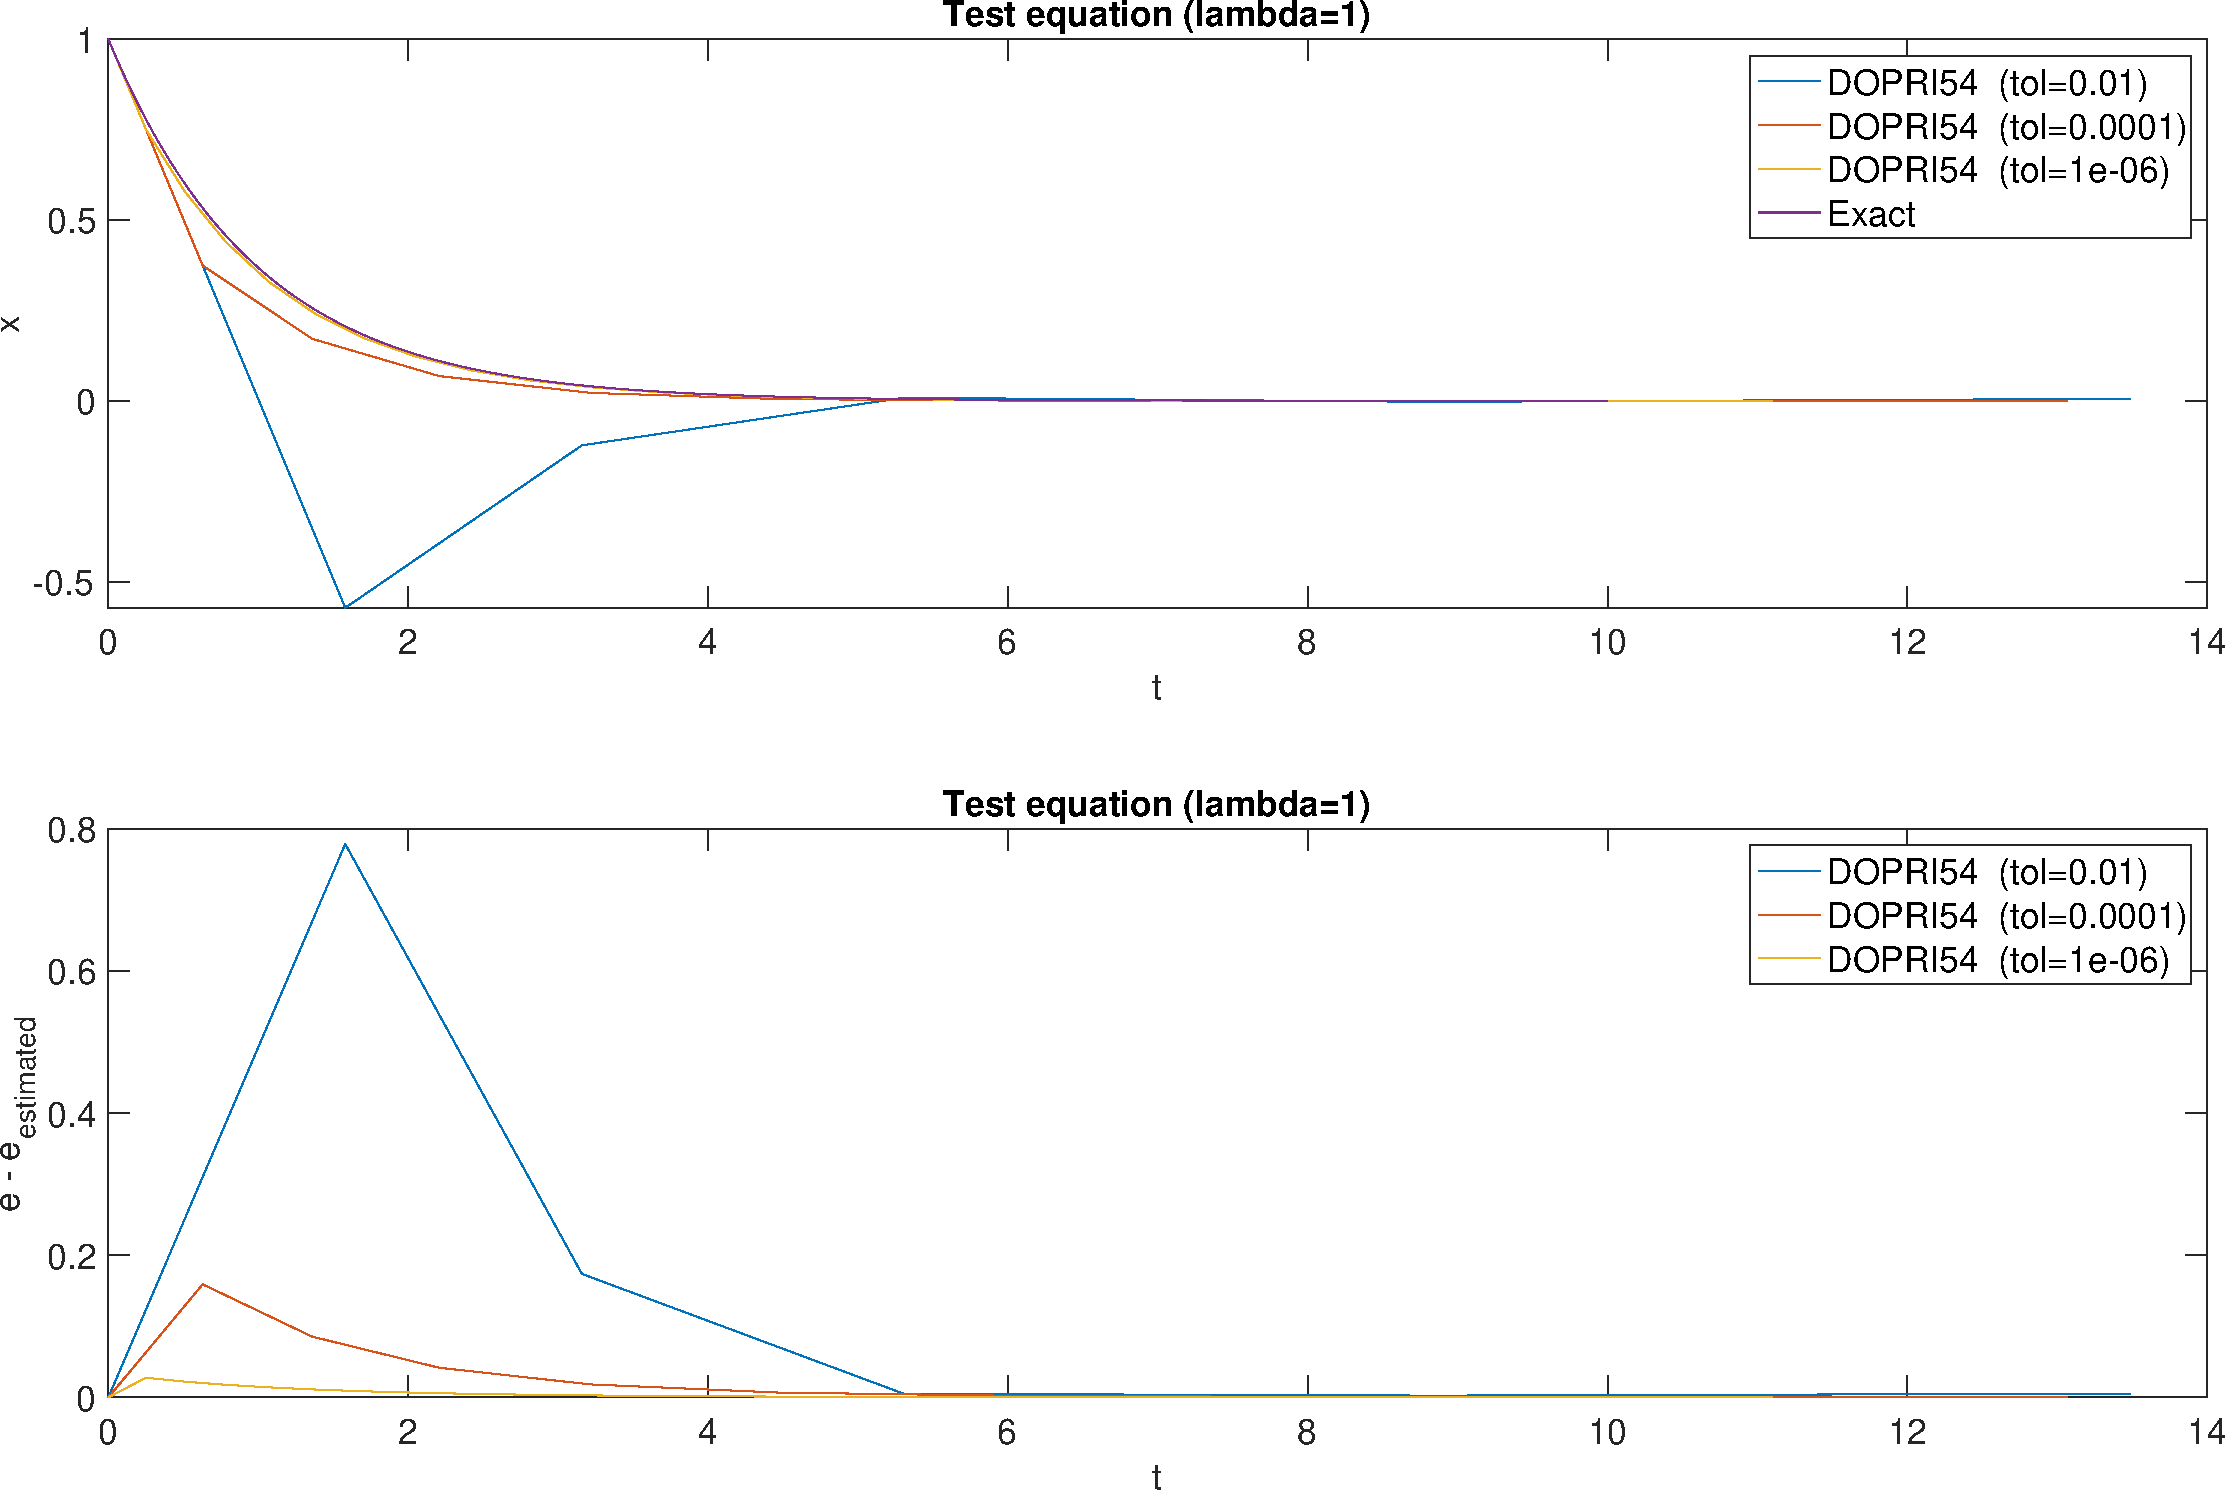
\includegraphics[width=0.7\textwidth]{plots/6_3a.pdf}
    \caption{DOPRI54 solution on the test equation with $\lambda=-1$.}
    \label{fig:6_3}
\end{figure}




\subsection{Van der Pol}

\subsection{Adiabatic Continuous Stirred Tank Reactor}

\subsection{Comparison with ode45}





























\newcolumntype{L}{>{$}l<{$}} % math-mode version of "l" column type
\begin{table}[htbp]
\label{tab:constants}
\caption{Table summarising the constants used in the CSTR model}
\centering
\begin{tabular}{lLLL}
\hline
Density                  & \rho       & 1.0       & kg/L            \\
Heat capacity            & c_P        & 4.186     & kJ/(kg \cdot K) \\
Arrhenius constant       & k_0        & exp(24.6) & L/(mol \cdot s) \\
Activation energy        & E_a/R      & 8500      & K               \\
Reaction enthalpy        & \Delta H_r & -560      & kJ/mol          \\
Reactor volume           & V          & 0.105     & L               \\
Inlet concentration of A & C_{A,in}   & 1.6/2     & mol/L           \\
Inlet concentration of B & C_{B,in}   & 2.4/2     & mol/L           \\
Inlet temperature        & T_{in}     & 273.65    & K               \\  \hline
\end{tabular}
\end{table}